%%%%%%%%%%%%%%%%%%%%%%%%%%%%%%%%%%%%%%%%%
% Programming/Coding Assignment
% LaTeX Template
%
% This template has been downloaded from:
% http://www.latextemplates.com
%
% Original author:
% Ted Pavlic (http://www.tedpavlic.com)
%
% Note:
% The \lipsum[#] commands throughout this template generate dummy text
% to fill the template out. These commands should all be removed when 
% writing assignment content.
%
% This template uses a Perl script as an example snippet of code, most other
% languages are also usable. Configure them in the "CODE INCLUSION 
% CONFIGURATION" section.
%
%%%%%%%%%%%%%%%%%%%%%%%%%%%%%%%%%%%%%%%%%

%----------------------------------------------------------------------------------------
%	PACKAGES AND OTHER DOCUMENT CONFIGURATIONS
%----------------------------------------------------------------------------------------

\documentclass{article}

\usepackage{fancyhdr} % Required for custom headers
\usepackage{lastpage} % Required to determine the last page for the footer
\usepackage{extramarks} % Required for headers and footers
\usepackage[usenames,dvipsnames]{color} % Required for custom colors
\usepackage{graphicx} % Required to insert images
\usepackage{listings} % Required for insertion of code
\usepackage{courier} % Required for the courier font
\usepackage{lipsum} % Used for inserting dummy 'Lorem ipsum' text into the template
\usepackage{setspace}
\usepackage{color}
\usepackage{comment}
\usepackage{caption}

\usepackage{hyperref}
\usepackage{natbib}
\usepackage{underscore}
\usepackage{subfigure}


\hypersetup{
    colorlinks=true,
    linkcolor=blue,
    filecolor=magenta,      
    urlcolor=cyan,
    breaklinks=true
}

%\usepackage[]{algorithm2e}
\usepackage{pdfpages}




%For python inclusion (http://widerin.org/blog/syntax-highlighting-for-python-scripts-in-latex-documents)
\definecolor{Code}{rgb}{0,0,0}
\definecolor{Decorators}{rgb}{0.5,0.5,0.5}
\definecolor{Numbers}{rgb}{0.5,0,0}
\definecolor{MatchingBrackets}{rgb}{0.25,0.5,0.5}
\definecolor{Keywords}{rgb}{0,0,1}
\definecolor{self}{rgb}{0,0,0}
\definecolor{Strings}{rgb}{0,0.63,0}
\definecolor{Comments}{rgb}{0,0.63,1}
\definecolor{Backquotes}{rgb}{0,0,0}
\definecolor{Classname}{rgb}{0,0,0}
\definecolor{FunctionName}{rgb}{0,0,0}
\definecolor{Operators}{rgb}{0,0,0}
\definecolor{Background}{rgb}{0.98,0.98,0.98}

% Margins
\topmargin=-0.45in
\evensidemargin=0in
\oddsidemargin=0in
\textwidth=6.5in
\textheight=9.0in
\headsep=0.25in

\linespread{1.1} % Line spacing

% Set up the header and footer
\pagestyle{fancy}
\lhead{\hmwkAuthorName} % Top left header
%\chead{\hmwkClass\ (\hmwkClassInstructor\ \hmwkClassTime): \hmwkTitle} % Top center head
\chead{\hmwkClass\ (\hmwkClassInstructor): \hmwkTitle} % Top center head
\rhead{\firstxmark} % Top right header
\lfoot{\lastxmark} % Bottom left footer
\cfoot{} % Bottom center footer
\rfoot{Page\ \thepage\ of\ \protect\pageref{LastPage}} % Bottom right footer
\renewcommand\headrulewidth{0.4pt} % Size of the header rule
\renewcommand\footrulewidth{0.4pt} % Size of the footer rule

\setlength\parindent{0pt} % Removes all indentation from paragraphs

%----------------------------------------------------------------------------------------
%	CODE INCLUSION CONFIGURATION
%----------------------------------------------------------------------------------------

\definecolor{MyDarkGreen}{rgb}{0.0,0.4,0.0} % This is the color used for comments
\lstloadlanguages{Perl} % Load Perl syntax for listings, for a list of other languages supported see: ftp://ftp.tex.ac.uk/tex-archive/macros/latex/contrib/listings/listings.pdf
\lstset{language=Perl, % Use Perl in this example
        frame=single, % Single frame around code
        basicstyle=\small\ttfamily, % Use small true type font
        keywordstyle=[1]\color{Blue}\bf, % Perl functions bold and blue
        keywordstyle=[2]\color{Purple}, % Perl function arguments purple
        keywordstyle=[3]\color{Blue}\underbar, % Custom functions underlined and blue
        identifierstyle=, % Nothing special about identifiers                                         
        commentstyle=\usefont{T1}{pcr}{m}{sl}\color{MyDarkGreen}\small, % Comments small dark green courier font
        stringstyle=\color{Purple}, % Strings are purple
        showstringspaces=false, % Don't put marks in string spaces
        tabsize=5, % 5 spaces per tab
        %
        % Put standard Perl functions not included in the default language here
        morekeywords={rand},
        %
        % Put Perl function parameters here
        morekeywords=[2]{on, off, interp},
        %
        % Put user defined functions here
        morekeywords=[3]{test},
       	%
        morecomment=[l][\color{Blue}]{...}, % Line continuation (...) like blue comment
        numbers=left, % Line numbers on left
        firstnumber=1, % Line numbers start with line 1
        numberstyle=\tiny\color{Blue}, % Line numbers are blue and small
        stepnumber=5 % Line numbers go in steps of 5
}

% Creates a new command to include a perl script, the first parameter is the filename of the script (without .pl), the second parameter is the caption
\newcommand{\perlscript}[2]{
\begin{itemize}
\item[]\lstinputlisting[caption=#2,label=#1]{#1.pl}
\end{itemize}
}


%----------------------------------------------------------------------------------------
%	DOCUMENT STRUCTURE COMMANDS
%	Skip this unless you know what you're doing
%----------------------------------------------------------------------------------------

% Header and footer for when a page split occurs within a problem environment
\newcommand{\enterProblemHeader}[1]{
\nobreak\extramarks{#1}{#1 continued on next page\ldots}\nobreak
\nobreak\extramarks{#1 (continued)}{#1 continued on next page\ldots}\nobreak
}

% Header and footer for when a page split occurs between problem environments
\newcommand{\exitProblemHeader}[1]{
\nobreak\extramarks{#1 (continued)}{#1 continued on next page\ldots}\nobreak
\nobreak\extramarks{#1}{}\nobreak
}

\setcounter{secnumdepth}{0} % Removes default section numbers
\newcounter{homeworkProblemCounter} % Creates a counter to keep track of the number of problems

\newcommand{\homeworkProblemName}{}
\newenvironment{homeworkProblem}[1][Problem \arabic{homeworkProblemCounter}]{ % Makes a new environment called homeworkProblem which takes 1 argument (custom name) but the default is "Problem #"
\stepcounter{homeworkProblemCounter} % Increase counter for number of problems
\renewcommand{\homeworkProblemName}{#1} % Assign \homeworkProblemName the name of the problem
\section{\homeworkProblemName} % Make a section in the document with the custom problem count
\enterProblemHeader{\homeworkProblemName} % Header and footer within the environment
}{
\exitProblemHeader{\homeworkProblemName} % Header and footer after the environment
}

\newcommand{\problemAnswer}[1]{ % Defines the problem answer command with the content as the only argument
\noindent\framebox[\columnwidth][c]{\begin{minipage}{0.98\columnwidth}#1\end{minipage}} % Makes the box around the problem answer and puts the content inside
}

\newcommand{\homeworkSectionName}{}
\newenvironment{homeworkSection}[1]{ % New environment for sections within homework problems, takes 1 argument - the name of the section
\renewcommand{\homeworkSectionName}{#1} % Assign \homeworkSectionName to the name of the section from the environment argument
\subsection{\homeworkSectionName} % Make a subsection with the custom name of the subsection
\enterProblemHeader{\homeworkProblemName\ [\homeworkSectionName]} % Header and footer within the environment
}{
\enterProblemHeader{\homeworkProblemName} % Header and footer after the environment
}

%----------------------------------------------------------------------------------------
%	NAME AND CLASS SECTION
%----------------------------------------------------------------------------------------

\newcommand{\hmwkTitle}{Assignment\ \#8 } % Assignment title
%\newcommand{\hmwkDueDate}{Monday,\ January\ 1,\ 2012} % Due date
\newcommand{\hmwkClass}{Introduction to Web Science} % Course/class
%\newcommand{\hmwkClassTime}{10:30am} % Class/lecture time
\newcommand{\hmwkClassInstructor}{Dr. Nelson} % Teacher/lecturer
\newcommand{\hmwkAuthorName}{Alexander Nwala} % Your name

%----------------------------------------------------------------------------------------
%	TITLE PAGE
%----------------------------------------------------------------------------------------

\title{
\vspace{2in}
\textmd{\textbf{\hmwkClass:\ \hmwkTitle}}\\
%\normalsize\vspace{0.1in}\small{Due\ on\ \hmwkDueDate}\\
%\vspace{0.1in}\large{\textit{\hmwkClassInstructor\ \hmwkClassTime}}
\vspace{0.1in}\large{\textit{\hmwkClassInstructor}}
\vspace{3in}
}

\author{\textbf{\hmwkAuthorName}}
\date{Thursday, November 13, 2014} % Insert date here if you want it to appear below your name

%----------------------------------------------------------------------------------------

\begin{document}

\maketitle



%----------------------------------------------------------------------------------------
%	TABLE OF CONTENTS
%----------------------------------------------------------------------------------------

%\setcounter{tocdepth}{1} % Uncomment this line if you don't want subsections listed in the ToC

\newpage
\tableofcontents
\newpage

%----------------------------------------------------------------------------------------
%	PROBLEM 1
%----------------------------------------------------------------------------------------

% To have just one problem per page, simply put a \clearpage after each problem

\begin{homeworkProblem}

The goal of this project is to use the basic recommendation principles
we have learned for user-collected data. You will modify the code
given to you which performs movie recommendations from the MovieLense
data sets.

The MovieLense data sets were collected by the GroupLens Research
Project at the University of Minnesota during the seven-month period
from September 19th, 1997 through April 22nd, 1998. It is available
for download from \url{http://www.grouplens.org/node/73}\\

There are three files which we will use:\\

1.  u.data: 100,000 ratings by 943 users on 1,682 movies. Each
user has rated at least 20 movies. Users and items are numbered
consecutively from 1. The data is randomly ordered. This is a tab
separated list of

\begin{verbatim}
user id | item id | rating | timestamp
\end{verbatim}

The time stamps are unix seconds since 1/1/1970 UTC.\\

Example:

\begin{verbatim}
196 242 3   881250949
186 302 3   891717742
22  377 1   878887116
244 51  2   880606923
166 346 1   886397596
298 474 4   884182806
115 265 2   881171488
\end{verbatim}

2.  u.item: Information about the 1,682 movies. This is a tab
separated list of

\begin{verbatim}
movie id | movie title | release date | video release date | IMDb URL 
| unknown | Action | Adventure | Animation |Children's | Comedy | Crime 
| Documentary | Drama | Fantasy | Film-Noir | Horror | Musical | Mystery 
| Romance | Sci-Fi | Thriller | War | Western |
\end{verbatim}

The last 19 fields are the genres, a 1 indicates the movie is of
that genre, a 0 indicates it is not; movies can be in several genres
at once. The movie ids are the ones used in the u.data data set.

Example:

\begin{verbatim}
161|Top Gun (1986)|01-Jan-1986||http://us.imdb.comMtitleexact?
Top%20Gun%20(1986)|0|1|0|0|0|0|0|0|0|0|0|0|0|0|1|0|0|0|0
162|On Golden Pond (1981)|01-Jan-1981|
|http://us.imdb.com/M/title-exact?On%20Golden%20Pond%20(1981)
|0|0|0|0|0|0|0|0|1|0|0|0|0|0|0|0|0|0|0
163|Return of the Pink Panther, The (1974)|01-Jan-1974|
|http://us.imdb.com/M/titleexact?Return%20of%20the%20Pink%20Panther,
%20The%20(1974)|0|0|0|0|0|1|0|0|0|0|0|0|0|0|0|0|0|0|0
\end{verbatim}

3.  u.user: Demographic information about the users. This is a tab
separated list of:

\begin{verbatim}
user id | age | gender | occupation | zip code
\end{verbatim}

The user ids are the ones used in the u.data data set.

Example:

\begin{verbatim}
1|24|M|technician|85711 
2|53|F|other|94043 
3|23|M|writer|32067 
4|24|M|technician|43537 
5|33|F|other|15213
\end{verbatim}

The code for reading from the u.data and u.item files and creating
recommendations is described in the book Programming Collective
Intelligence (check email for more details). You are to modify
recommendations.py to answer the following questions. Each question your
program answers correctly will award you 1 point.\\

1.  What 5 movies have the highest average ratings? Show the movies
and their ratings sorted by their average ratings.\\

2.  What 5 movies received the most ratings? Show the movies and
the number of ratings sorted by number of ratings.\\

3.  What 5 movies were rated the highest on average by women? Show
the movies and their ratings sorted by ratings.\\

4.  What 5 movies were rated the highest on average by men? Show
the movies and their ratings sorted by ratings.\\

5.  What movie received ratings most like Top Gun? Which movie
received ratings that were least like Top Gun (negative correlation)?\\

6.  Which 5 raters rated the most films? Show the raters' IDs and
the number of films each rated.\\

7.  Which 5 raters most agreed with each other? Show the raters'
IDs and Pearson's r, sorted by r.\\

8.  Which 5 raters most disagreed with each other (negative
correlation)? Show the raters' IDs and Pearson's r, sorted by r.\\

9.  What movie was rated highest on average by men over 40? By men
under 40?\\

10. What movie was rated highest on average by women over 40? By
women under 40?\\

Your output should clearly indicate the answers from the question
you answered.  Provide any relevant discussion.\\

%\problemAnswer
%{
    \begin{verbatim}\end{verbatim}
    \textbf{SOLUTIONS}\\


    The solutions for these problem are outlined by the following steps:
    \begin{enumerate}

    \item \textbf{Solution 1 - Aggregate movie and rater data:} This was achieved by reading u.item and u.data and bringing items with common IDs into the same structure in order to produce the following lists

    \begin{verbatim}
        movies: <movie id, (movie title, ratingsArray)>

        aggregateMovieData: [ (movie id, movie title, 
        average movie rating, number of ratings) ]

        aggregateUserData: [ (rater id, gender, age,
        {'movie id': movie rating}) ]
    \end{verbatim}

    as outlined in Listing 1. Thereafter, a call to to getHighestRatedMovies(aggregateMovies, 10) (Listing 2.) produced Table 1. 

   

    \lstinputlisting[breaklines=true, caption=Aggregate Movie and Rater data]{aggregateDataSnippet.py}
    \lstinputlisting[breaklines=true, caption=Get Highest Rated Movies]{getHighestRatedMoviesSnippet.py}

    \item \textbf{Solution 2:} Based upon Listing 1 (Aggregated data), a call to getMostRatedMovies(aggregateMovies, 5) (Listing 3.), produced Table 2.

    \lstinputlisting[breaklines=true, caption=Most Rated Movies]{getMostRatedMoviesSnippet.py}

    \begin{table}
    \caption{Arbitrary Subset of Highest Rated Movies} % title of Table
    \centering % used for centering table
    \begin{tabular}{c | c | c | c } % centered columns (4 columns)
    \hline\hline %inserts double horizontal lines
    ITEM & MOVIE-ID & MOVIE-NAME & RATING \\ [0.5ex] % inserts table 
    %heading
    \hline \hline% inserts single horizontal line
    1   &   1653    &   Entertaining Angels: The Dorothy Day Story (1996) & 5.0 \\ \hline
    2   &   1500    &   Santa with Muscles (1996) & 5.0 \\ \hline
    3   &   814    &   Great Day in Harlem, A (1994) & 5.0 \\ \hline
    4   &   1122    &   They Made Me a Criminal (1939)  & 5.0 \\ \hline
    5 & 1536 & Aiqing wansui (1994) & 5.0 \\ [1ex] 
    \hline %inserts single line
    \end{tabular}
    \label{table:nonlin} % is used to refer this table in the text
    \end{table}

    \begin{table}
    \caption{Most Rated Movies} % title of Table
    \centering % used for centering table
    \begin{tabular}{c | c | c | c } % centered columns (4 columns)
    \hline\hline %inserts double horizontal lines
    ITEM & MOVIE-ID & MOVIE-NAME & RATINGS COUNT \\ [0.5ex] % inserts table 
    %heading
    \hline \hline% inserts single horizontal line
    1   &   50    &   Star Wars (1977) & 583 \\ \hline
    2   &   258    &   Contact (1997) & 509 \\ \hline
    3   &   100    &   Fargo (1996) & 508 \\ \hline
    4   &   181    &   Return of the Jedi (1983)  & 507 \\ \hline
    5 & 294 & Liar Liar (1997) & 485 \\ [1ex] 
    \hline %inserts single line
    \end{tabular}
    \label{table:nonlin} % is used to refer this table in the text
    \end{table}

    \begin{table}
    \caption{Arbitrary Subset of Highest Rated Movies by Women} % title of Table
    \centering % used for centering table
    \begin{tabular}{c | c | c | c} % centered columns (4 columns)
    \hline\hline %inserts double horizontal lines
    ITEM & MOVIE-NAME & RATING \\ [0.5ex] % inserts table 
    %heading
    \hline \hline% inserts single horizontal line
    1   &   Everest (1998)   &   5.0 \\ \hline
    2   &   Someone Else's America (1995)   &   5.0 \\ \hline
    3   &   Foreign Correspondent (1940)    &   5.0 \\ \hline
    4   &   Visitors, The (Visiteurs, Les) (1993)    &  5.0 \\ \hline
    5 & Stripes (1981) & 5.0 \\ [1ex] 
    \hline %inserts single line
    \end{tabular}
    \label{table:nonlin} % is used to refer this table in the text
    \end{table}

    \begin{table}
    \caption{Arbitrary Subset of Highest Rated Movies by Men} % title of Table
    \centering % used for centering table
    \begin{tabular}{c | c | c | c} % centered columns (4 columns)
    \hline\hline %inserts double horizontal lines
    ITEM & MOVIE-NAME & RATING \\ [0.5ex] % inserts table 
    %heading
    \hline \hline% inserts single horizontal line
    1   &   Entertaining Angels: The Dorothy Day Story (1996)   &   5.0 \\ \hline
    2   &   Letter From Death Row, A (1998)   &   5.0 \\ \hline
    3   &   Hugo Pool (1997) 5.0    &   5.0 \\ \hline
    4   &   Santa with Muscles (1996)   &  5.0 \\ \hline
    5 & Leading Man, The (1996) & 5.0 \\ [1ex] 
    \hline %inserts single line
    \end{tabular}
    \label{table:nonlin} % is used to refer this table in the text
    \end{table}

    \item \textbf{Solution 3 - Aggregate male and female data:} Similar to aggregating movie data, getFemaleAndMaleData() (Listing 4.) produces 2 lists - 1 for male, the other for female raters. Thereafter, the following call getHighestRatedMoviesByMenOrWomen(aggregateUsersFemale, 5, movies) (Listing 4.) produced Table 3.

    \lstinputlisting[breaklines=true, caption=Aggregate Male and Female and get Highest Rated]{getMaleAndFemaleDataSnippet.py}

    \item \textbf{Solution 4:} Similar to solution 3, a call getHighestRatedMoviesByMenOrWomen(aggregateUsersMale, 5, movies) (Listing 4.) produced Table 4.

    \item \textbf{Solution 5:}

        \begin{enumerate}
            \item \textbf{Populate movie and user dictionary:} This was done through the MovieLens's loadMovieLens() method (Listing 5.) with a single modification - the movies dictionary was indexed with the movie id instead of the movie title due to duplicate title entries.
            
            \item \textbf{Calculate one vs rest similarity:} This was also done through a slightly modified MovieLen's calculateSimilarItems() method by the following calls:

            \begin{verbatim}

            # call for most correlated
            mostSimilarToTopGun = calculateSimilarItems
            ( prefs=prefs,
              simMeasure=sim_pearson,
              n=5,
              reverseSimilarityFlag=True,
              transformMatrixFlag=True
            )

            # call for least correlated
            leastSimilarToTopGun = calculateSimilarItems
            ( prefs=prefs, 
              simMeasure=sim_pearson, 
              n=5, 
              reverseSimilarityFlag=False,
              transformMatrixFlag=True
            )

            \end{verbatim}

            The modification allowed the option of passing the similarity measure as a function argument, as well as sorting the list in ascending or descending order. Finally the resultant similarity dictionary was indexed with Top Gun's movie id (161) to produce Table 5 and 6.

            \lstinputlisting[breaklines=true, caption=Movies Most/Least Similar to Top Gun]{mostCorrelatedToTopGunSnippet.py}
        \end{enumerate}

        \begin{table}
        \caption{Arbitrary Subset of Movies most Correlated to Top Gun} % title of Table
        \centering % used for centering table
        \begin{tabular}{c | c | c | c} % centered columns (4 columns)
        \hline\hline %inserts double horizontal lines
        ITEM & MOVIE-NAME & CORRELATION COEFFICIENT \\ [0.5ex] % inserts table 
        %heading
        \hline \hline% inserts single horizontal line
        1   &   King of the Hill (1993)   &   1.0 \\ \hline
        2   &   Shiloh (1997) &   1.0 \\ \hline
        3   &   Bhaji on the Beach (1993) &   1.0 \\ \hline
        4   &   Dangerous Ground (1997) &  1.0 \\ \hline
        5 & Hear My Song (1991) & 1.0 \\ [1ex] 
        \hline %inserts single line
        \end{tabular}
        \label{table:nonlin} % is used to refer this table in the text
        \end{table}

        \begin{table}
        \caption{Arbitrary Subset of Movies least Correlated to Top Gun} % title of Table
        \centering % used for centering table
        \begin{tabular}{c | c | c | c} % centered columns (4 columns)
        \hline\hline %inserts double horizontal lines
        ITEM & MOVIE-NAME & CORRELATION COEFFICIENT \\ [0.5ex] % inserts table 
        %heading
        \hline \hline% inserts single horizontal line
        1   &   Babysitter, The (1995) &   -1.0 \\ \hline
        2   &   Telling Lies in America (1997) &   -1.0 \\ \hline
        3   &   Switchback (1997) &   -1.0 \\ \hline
        4   &   Carried Away (1996) &  -1.0 \\ \hline
        5 & Two Much (1996) & -1.0 \\ [1ex] 
        \hline %inserts single line
        \end{tabular}
        \label{table:nonlin} % is used to refer this table in the text
        \end{table}

        \begin{table}
        \caption{Highest Movie Raters} % title of Table
        \centering % used for centering table
        \begin{tabular}{c | c | c | c} % centered columns (4 columns)
        \hline\hline %inserts double horizontal lines
        ITEM & RATER-ID & No. RATINGS \\ [0.5ex] % inserts table 
        %heading
        \hline \hline% inserts single horizontal line
        1   &   405 &  737 \\ \hline
        2   &   655 &  685 \\ \hline
        3   &   13 &   636 \\ \hline
        4   &   450 &  540 \\ \hline
        5 & 276  & 518 \\ [1ex] 
        \hline %inserts single line
        \end{tabular}
        \label{table:nonlin} % is used to refer this table in the text
        \end{table}

    \item \textbf{Solution 6 - get highest movie rater:} This was achieved through a simple counting function (Listing 6.), which produced Table 7.
    \lstinputlisting[breaklines=true, caption=Highest Movie Raters]{getHighestMovieRatersSnippet.py}

    \item \textbf{Solution 7:}

        \begin{enumerate}
            \item \textbf{Generate distance matrix:} This was achieved through a call to calculateSimilarItems() by passing a Euclidean distance (sim_distance) metric argument (Listing 5.):

            \begin{verbatim}
                #sort result from smallest distance to largest
                userSimilarityMatrix = calculateSimilarItems
                (
                    prefs=prefs, 
                    simMeasure=sim_distance, 
                    n=5, 
                    reverseSimilarityFlag=False, 
                    transformMatrixFlag=False
                )
                The result of this was written to hierarchicalClusterInput1.txt
            \end{verbatim}

            

            \item \textbf{Search for hierarchical cluster with 5 items:} This was achieved through Listing 7. By iteratively and incrementally generating hierarchical clusters. The search resulted in a clustering of 27 containing 5 raters: (551, 789, 814, 846, 881). Figure 1. outlines the dendogram.

            \begin{figure}

                \caption{Hierarchical Cluster with a Cluster of 5 Closest Raters (551, 789, 814, 846, 881)}
                \subfigure[Hierarchical Clustering]{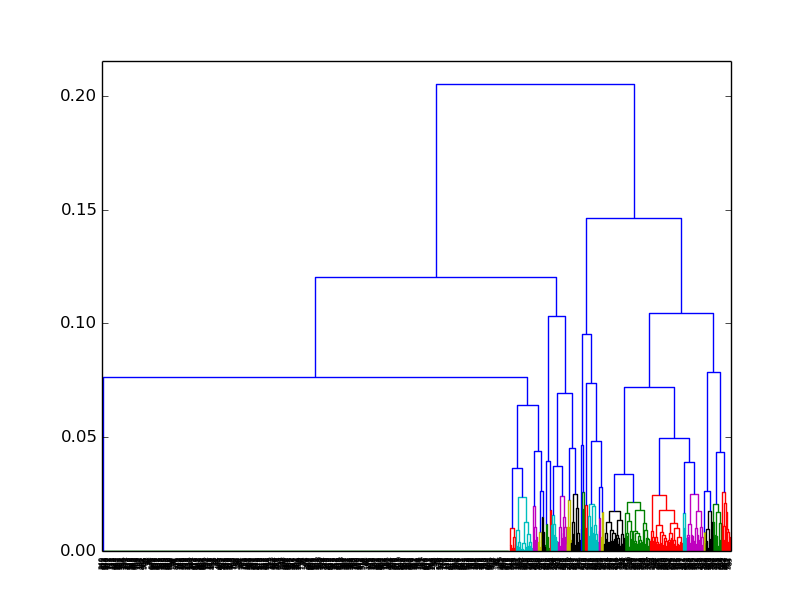
\includegraphics[width=\textwidth]{hCluster1.png}}

            \end{figure}

            \lstinputlisting[breaklines=true, caption=Hierarchical Clustering with Dendogram Plot]{hClusterSnippet.py}

            In order to get the average Pearson's r (sorted by r), Listing 8. computes pairwise Pearson similarity matrix for the 5 raters and calcuates the averages of each row, with the result outlined in Table 8.

            \lstinputlisting[breaklines=true, caption=Pearson's similarity for 5 raters]{pearsonPairwiseMatrixSnippet.py}

            \begin{table}[h]
            \caption{Pearson's Coefficient for 5 Similar Raters} % title of Table
            \centering % used for centering table
            \begin{tabular}{c | c | c | c} % centered columns (4 columns)
            \hline\hline %inserts double horizontal lines
            ITEM & RATER & CORRELATION COEFFICIENT \\ [0.5ex] % inserts table 
            %heading
            \hline \hline% inserts single horizontal line
            1   &   789 &  0.3316 \\ \hline
            2   &   881 &  0.2847 \\ \hline
            3   &   846 &   0.2545 \\ \hline
            4   &   551 &  0.0740 \\ \hline
            5 & 814  & 0.0566 \\ [1ex] 
            \hline %inserts single line
            \end{tabular}
            \label{table:nonlin} % is used to refer this table in the text
            \end{table}
        \end{enumerate}

        \item \textbf{Solution 8:} Solution 8 follows the same pathway (distance matrix, search clusterings) as solution 7 with the exception of the call:

        \begin{verbatim}
            #sort result from largest distance to smallest
            userSimilarityMatrix = calculateSimilarItems
            (   
                prefs=prefs,
                simMeasure=sim_distance, 
                n=5, 
                reverseSimilarityFlag=True, 
                transformMatrixFlag=False
            )

            The result of this was written to hierarchicalClusterInput2.txt
        \end{verbatim}

        The 5 raters who least agree are: (193, 206, 233, 302, 825). Table 9. was achieved in a similar fashion as solution 7.

        \begin{table}[h]
        \caption{Pearson's Coefficient for 5 least Similar Raters} % title of Table
        \centering % used for centering table
        \begin{tabular}{c | c | c | c} % centered columns (4 columns)
        \hline\hline %inserts double horizontal lines
        ITEM & RATER & CORRELATION COEFFICIENT \\ [0.5ex] % inserts table 
        %heading
        \hline \hline% inserts single horizontal line
        1   &   825 &  -0.2781 \\ \hline
        2   &   233 &  -0.0989 \\ \hline
        3   &   206 &   -0.0606 \\ \hline
        4   &   302 &  0.1550 \\ \hline
        5 &  193 & 0.2395 \\ [1ex] 
        \hline %inserts single line
        \end{tabular}
        \label{table:nonlin} % is used to refer this table in the text
        \end{table}

    \item \textbf{Solution 9:} By applying an age filter on the aggregate male data and using the result to query the aggregate movie data, Listing 9. gets the highest rated movies by men above/below 40 (Table 10 and 11.)


    \lstinputlisting[breaklines=true, caption=Highest Rated Movies By Men/Women Above/Below age]{moveshighestRatedMoviesByMenWomenAboveSnippet.py}


    \begin{table}[h]
    \caption{Arbitrary Subset of Highest Rated Movies by Men over 40} % title of Table
    \centering % used for centering table
    \begin{tabular}{c | c | c | c} % centered columns (4 columns)
    \hline\hline %inserts double horizontal lines
    ITEM & MOVIE-NAME & RATING \\ [0.5ex] % inserts table 
    %heading
    \hline \hline% inserts single horizontal line
    1   &   Great Day in Harlem, A (1994) &  5.0 \\ \hline
    2   &   Two or Three Things I Know About Her (1966) &  5.0 \\ \hline
    3   &   Aparajito (1956) &  5.0 \\ \hline
    4   &   Strawberry and Chocolate (Fresa y chocolate) (1993) &  5.0 \\ \hline
    5 & Little Princess, The (1939) & 5.0 \\ [1ex] 
    \hline %inserts single line
    \end{tabular}
    \label{table:nonlin} % is used to refer this table in the text
    \end{table}

    \begin{table}[h]
    \caption{Arbitrary Subset of Highest Rated Movies by Men under 40} % title of Table
    \centering % used for centering table
    \begin{tabular}{c | c | c | c} % centered columns (4 columns)
    \hline\hline %inserts double horizontal lines
    ITEM & MOVIE-NAME & RATING \\ [0.5ex] % inserts table 
    %heading
    \hline \hline% inserts single horizontal line
    1   &   Entertaining Angels: The Dorothy Day Story (1996) &  5.0 \\ \hline
    2   &   Letter From Death Row, A (1998) &  5.0 \\ \hline
    3   &   Hugo Pool (1997) &  5.0 \\ \hline
    4   &   Leading Man, The (1996) &  5.0 \\ \hline
    5 & Quiet Room, The (1996) & 5.0 \\ [1ex] 
    \hline %inserts single line
    \end{tabular}
    \label{table:nonlin} % is used to refer this table in the text
    \end{table}

    \item \textbf{Solution 10:} Solution 10 uses the same means as solution 9 to get the result highest rated movies by women above/below 40 with the exception of passing the getHighestRatedMoviesByMenOrWomenOverAge() (Listing 9.) and getHighestRatedMoviesByMenOrWomenUnderAge() (Listing 9.) the aggregate female data. Table 12 and 13. outlines the results.

    \begin{table}[h]
    \caption{Arbitrary Subset of Highest Rated Movies by Women over 40} % title of Table
    \centering % used for centering table
    \begin{tabular}{c | c | c | c} % centered columns (4 columns)
    \hline\hline %inserts double horizontal lines
    ITEM & MOVIE-NAME & RATING \\ [0.5ex] % inserts table 
    %heading
    \hline \hline% inserts single horizontal line
    1   &   In the Bleak Midwinter (1995) &  5.0 \\ \hline
    2   &   Foreign Correspondent (1940) &  5.0 \\ \hline
    3   &   Swept from the Sea (1997) &  5.0 \\ \hline
    4   &   Great Dictator, The (1940) &  5.0 \\ \hline
    5 & Balto (1995) The (1939) & 5.0 \\ [1ex] 
    \hline %inserts single line
    \end{tabular}
    \label{table:nonlin} % is used to refer this table in the text
    \end{table}

    \begin{table}[h]
    \caption{Arbitrary Subset of Highest Rated Movies by Women under 40} % title of Table
    \centering % used for centering table
    \begin{tabular}{c | c | c | c} % centered columns (4 columns)
    \hline\hline %inserts double horizontal lines
    ITEM & MOVIE-NAME & RATING \\ [0.5ex] % inserts table 
    %heading
    \hline \hline% inserts single horizontal line
    1   &   Nico Icon (1995) &  5.0 \\ \hline
    2   &   Backbeat (1993) &  5.0 \\ \hline
    3   &   Umbrellas of Cherbourg, The (Parapluies de Cherbourg, Les) (1964) &  5.0 \\ \hline
    4   &   Everest (1998) &  5.0 \\ \hline
    5 & Someone Else's America (1995) & 5.0 \\ [1ex] 
    \hline %inserts single line
    \end{tabular}
    \label{table:nonlin} % is used to refer this table in the text
    \end{table}

   
    \end{enumerate}

%}



\end{homeworkProblem}


%----------------------------------------------------------------------------------------

\end{document}